\documentclass[IN,11pt,twoside,openright,bachelor,english]{tumthesis}

\usepackage{packages}
\usepackage{IEEEtrantools}

\newcommand\toc{\relax}

\usepackage[backend=bibtex,style=ieee]{biblatex}
\usepackage{booktabs}
\usepackage{tabularx}
\usepackage{listings}

\usepackage{longtable}
\usepackage{tabu}
\usepackage{ltxtable}
\usepackage{url}
\usepackage[style=base]{caption}
\captionsetup{%
	font={rm,footnotesize},
	labelfont={sc},
}
\captionsetup[subfloat]{%
	font={rm,footnotesize},
	labelfont={rm},
}
\usepackage{subcaption}
\usepackage{nicefrac}
\usepackage{longtable}
\usepackage[hang]{footmisc}
\usepackage{blindtext}
\usepackage[printonlyused]{acronym}

\setlength\footnotemargin{5pt}

% Theorem environments
\newtheorem{definition}{Definition}
\newtheorem{theorem}{Theorem}
\newtheorem{example}{Example}
\newtheorem{lemma}{Lemma}


\usepackage{mdframed}
\newlength{\charwidth}
\setlength{\charwidth}{\widthof{\scriptsize\texttt{x}}}

\makeatletter
\newenvironment{moeplstborder}[2][]{%
\ifx#1\@empty\@empty%
	\edef\@margin{-1.5\baselineskip}%
\else%
	\edef\@margin{#1}%
\fi%
\vspace{-\baselineskip}
\begin{center}
\begin{minipage}{#2}
\begin{mdframed}[%
	topline=false,leftline=false,bottomline=false,rightline=true,
	linecolor=TUMRed!20,linewidth=\charwidth,
	innertopmargin=\@margin,innerbottommargin=-0.5\baselineskip,
	innerleftmargin=0pt,innerrightmargin=-\charwidth,
	userdefinedwidth=#2,
]%
}%
{%
\end{mdframed}%
\end{minipage}
\end{center}
}%
\makeatother


% \betreuer{Leander Seidlitz, Johannes Zirngibl}
% Needed for Bachelor's theses, Master's theses and IDP
\titleenglish{Development of a Framework for Retrieval of Parameters of the Starlink Dish}
\titlegerman{Entwurf eines Frameworks zur Informationsgewinnung von Parametern der Starlink Dish}
\author{Roberto Castellotti}
\supervisor{\chairhead}
% I am not sure what I should add here
\assistants{Dr.-Ing.~Stephan~M.~G\"unther\tlc{},%
Sebastian~Gallenmüller\tlc{}~B.\,Sc.}

% Only needed for dissertation
\chairman{\makebox[7cm]{\dotfill}}
\advisor{Prof.~Dr.-Ing.~Wolfgang~Utschick}

\courseofstudy{Electrical Engineering}

\date{September 15, 2016}

% Only for accepted disserations
%\date[November 15, 2021]{September 15, 2021} % [acceptance date]{hand-in date}

\location{Garching}

\setcounter{tocdepth}{2}

\addbibresource{bib/litnew.bib}
% Load late to avoid same identifier warning
\usepackage[colorlinks=false,pdfborder={0 0 0}]{hyperref}


\begin{document}

\pagenumbering{gobble}	
\maketitle%
\cleardoublepage


\begin{abstract} 
In this report we want to document our work and findings on Starlink based connections. 

We investigate whether Starlink-based connections result in a different routing of packets when reaching some geographically sparse targets, after that we move on analyzing whether the dish performs some buffering before relaying packets to satellite.

Lastly we analyzed satellites visible from a dish and, after developing a script to detect satellite handovers, we moved on trying to correlate  drops in bandwidth and satellite handovers, handovers don't seem to happen in a specific pattern nor are indicative of a drop in bandwidth. 
\end{abstract}


\begin{thanks}
\end{thanks}

\tableofcontents
\listoffigures
\listoftables

\startcontent

\chapter{Introduction}

Starlink is the largest Low Earth Orbiting, hereinafter LEO, satellite constellation managed by SpaceX aimed at providing internet broadband connection in the most remote and rural areas in the world while also issuing the service to people living in residential areas. LEO satellites orbit at around 550 Kms from earth, this leads to a low latency, SpaceX claims latency is around ~25 ms, from our experiments it is higher (~45ms) but it is still order of magnitudes lower than other satellite based solutions.  For the latter Starlink might not be the best solution, as probably their place is covered by a default connection which probably is way cheaper as the infrastructure is simpler to maintain and the fixed costs one has to substain are way less. This technology however makes night-and-day difference for people living in the most isolated places in the world. 
Satellite based internet connections have been around for several years, those are based on geostationary satellites,hereinafter GEOSAT, orbiting at around 35.000 kms, it is thus natural to expect high latency for a normal internet connection.
A generic GEOSAT connection averages around 600 ms for latency, this means in average Starlink does ~70 RTTs in the time a GEOSAT satellite does 1 RTT.

From a customer perspective using Starlink is straightforward, after the customer orders his hardware package he only needs to plug the satellite dish he receives (see Figure \ref{fig:dish}) and position it in a place where the dish has clear access to the sky, after that plugging in the router is enough to start browsing the internet.

On a more technical note what is happening is packets from a local device go through the dish and they are relayed to a nearby satellite and they are sent to a ground station in view, from that point onwards packets are routed normally through the internet.

SpaceX is also experimenting with Inter Satellite Links, this would allow satellites to comunicate between each other without resorting to ground local stations. This is crucial for the maritime version of the Starlink kit, moreover it might be possible that using laser links is faster than fiber on Earth, thus providing lower latencies connection to everyone, as reported by Elon Musk himself \cite{tweet}.

\begin{figure}
	\label{fig:gs}
	\centering
	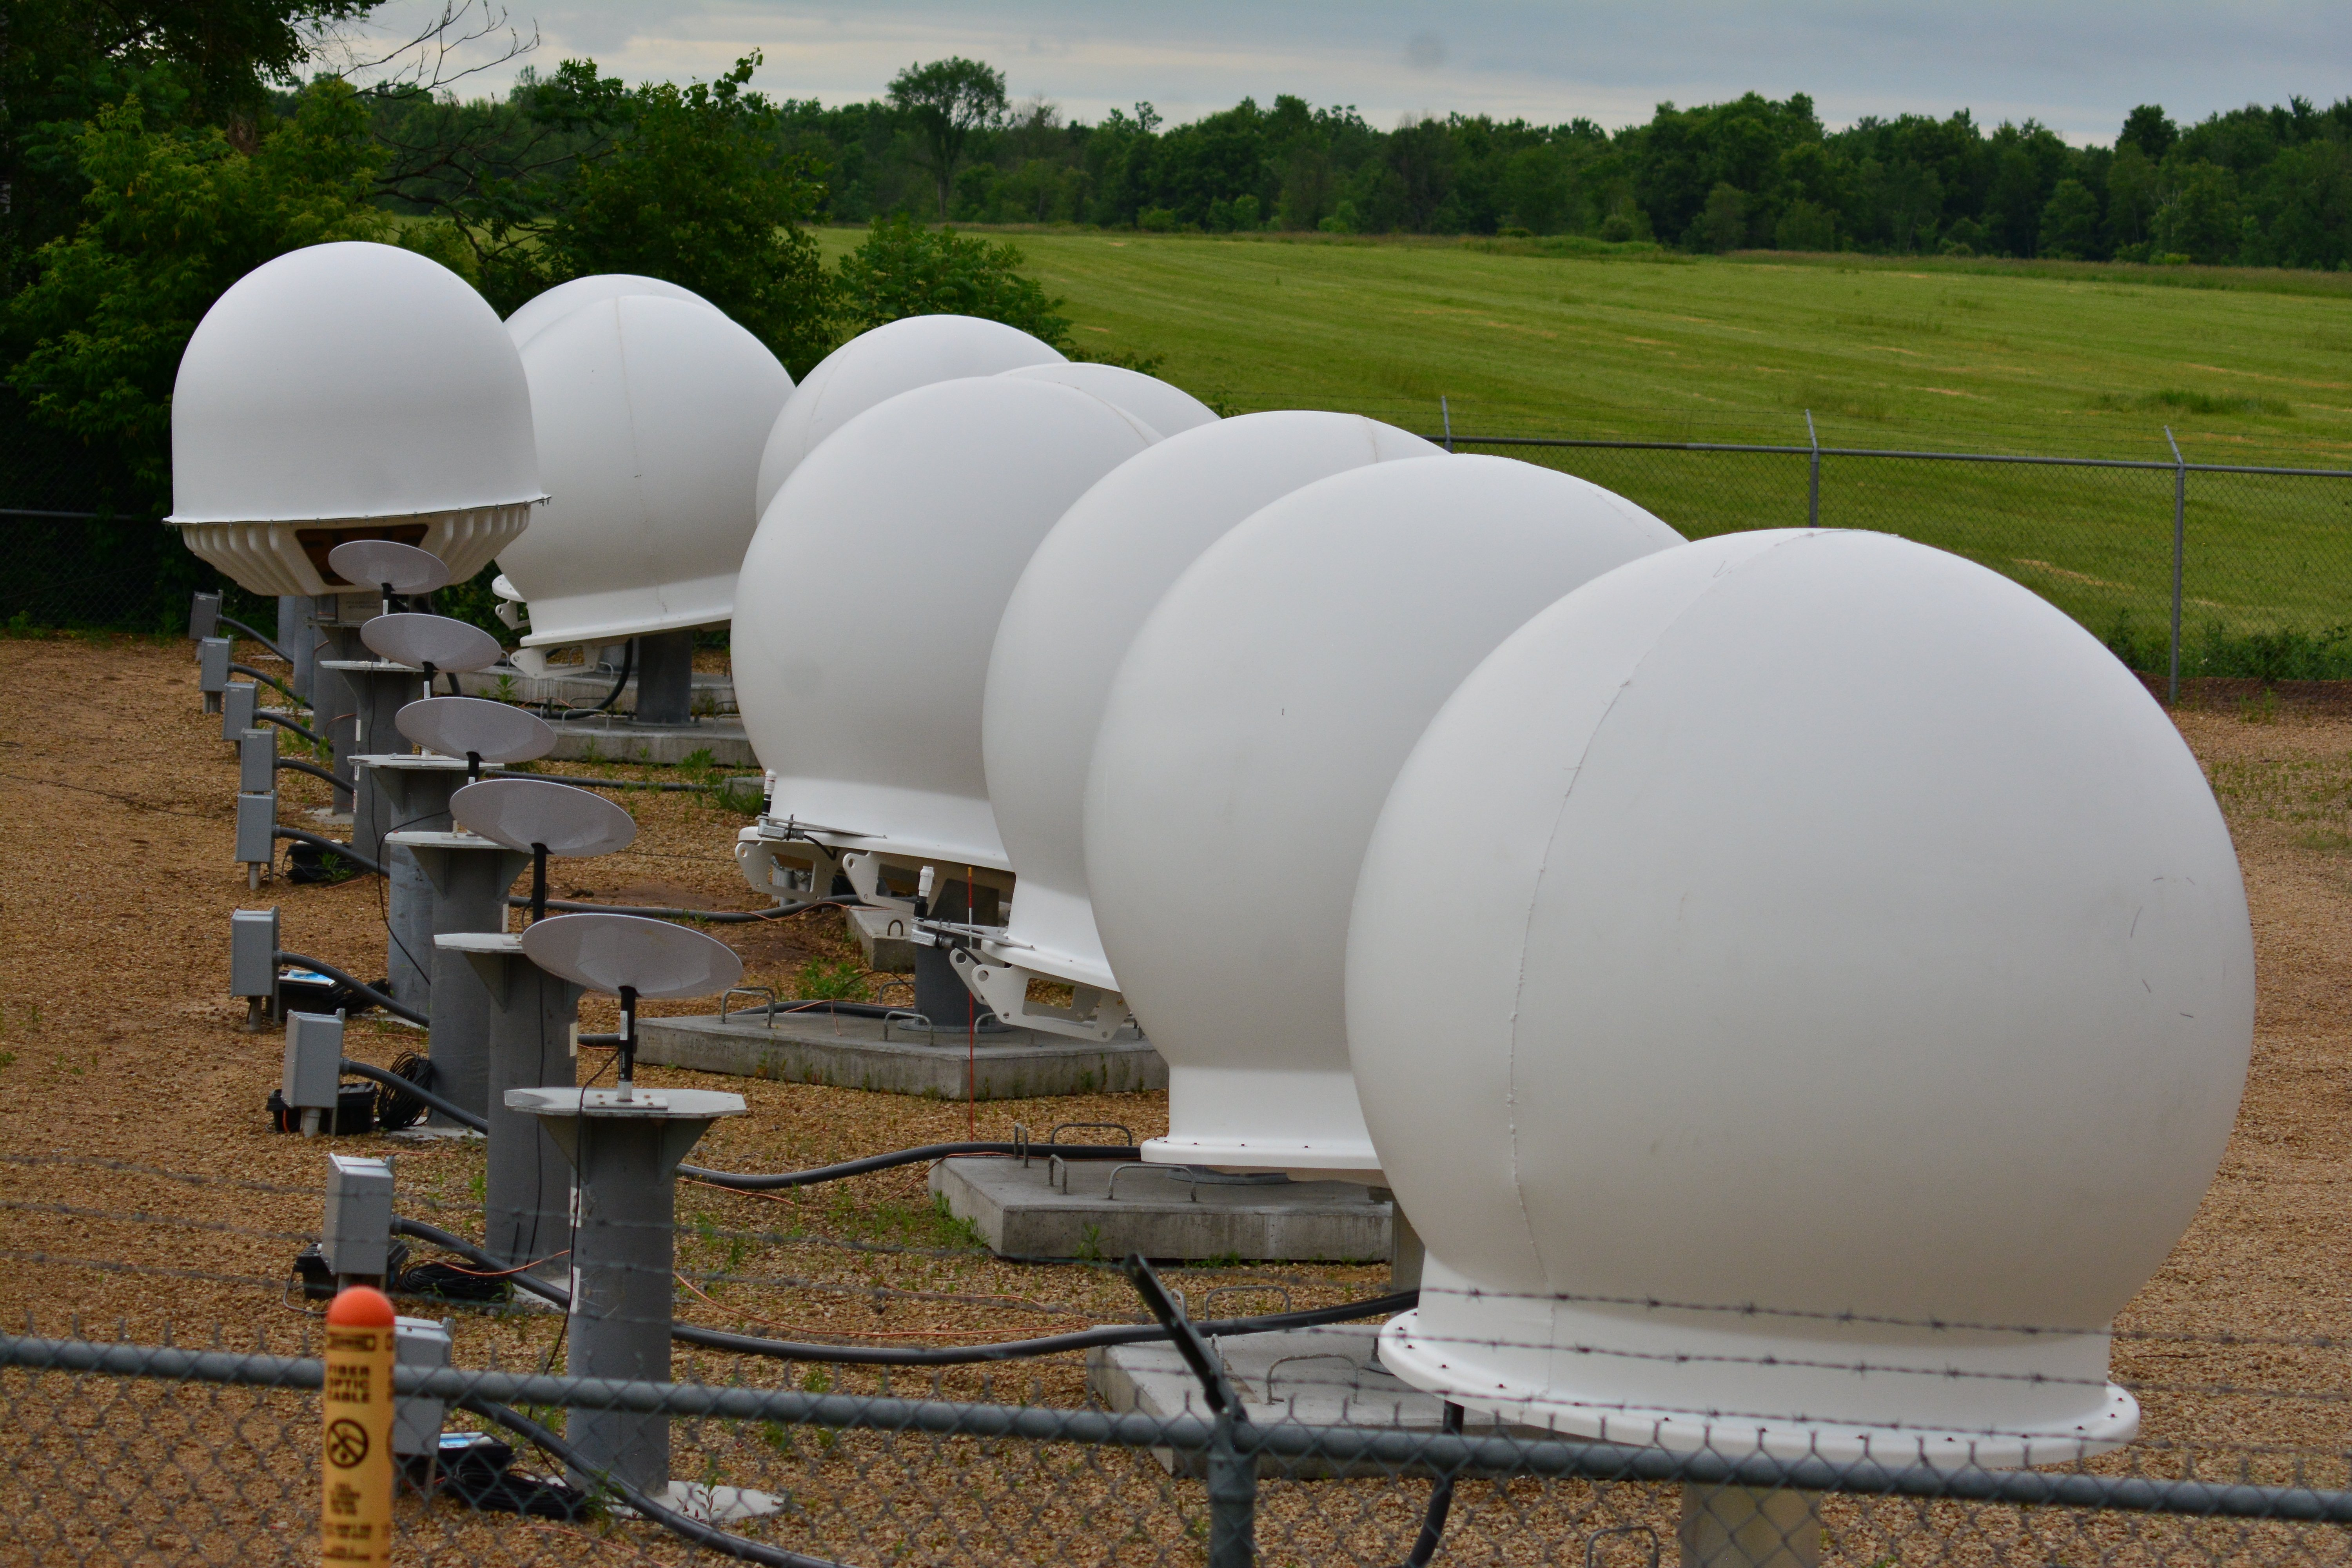
\includegraphics[width=0.6\columnwidth]{img/ground-station.jpeg}
	\caption{A sample ground station, from \href{https://www.reddit.com/r/SpaceXLounge/comments/hcf4t5/prototype_starlink_terminal_closeups_merrillan_wi/}{u/darkpenguin22, posted on r/SpaceXLounge}}
\end{figure}

\begin{figure}
	\label{fig:dish}
	\centering
	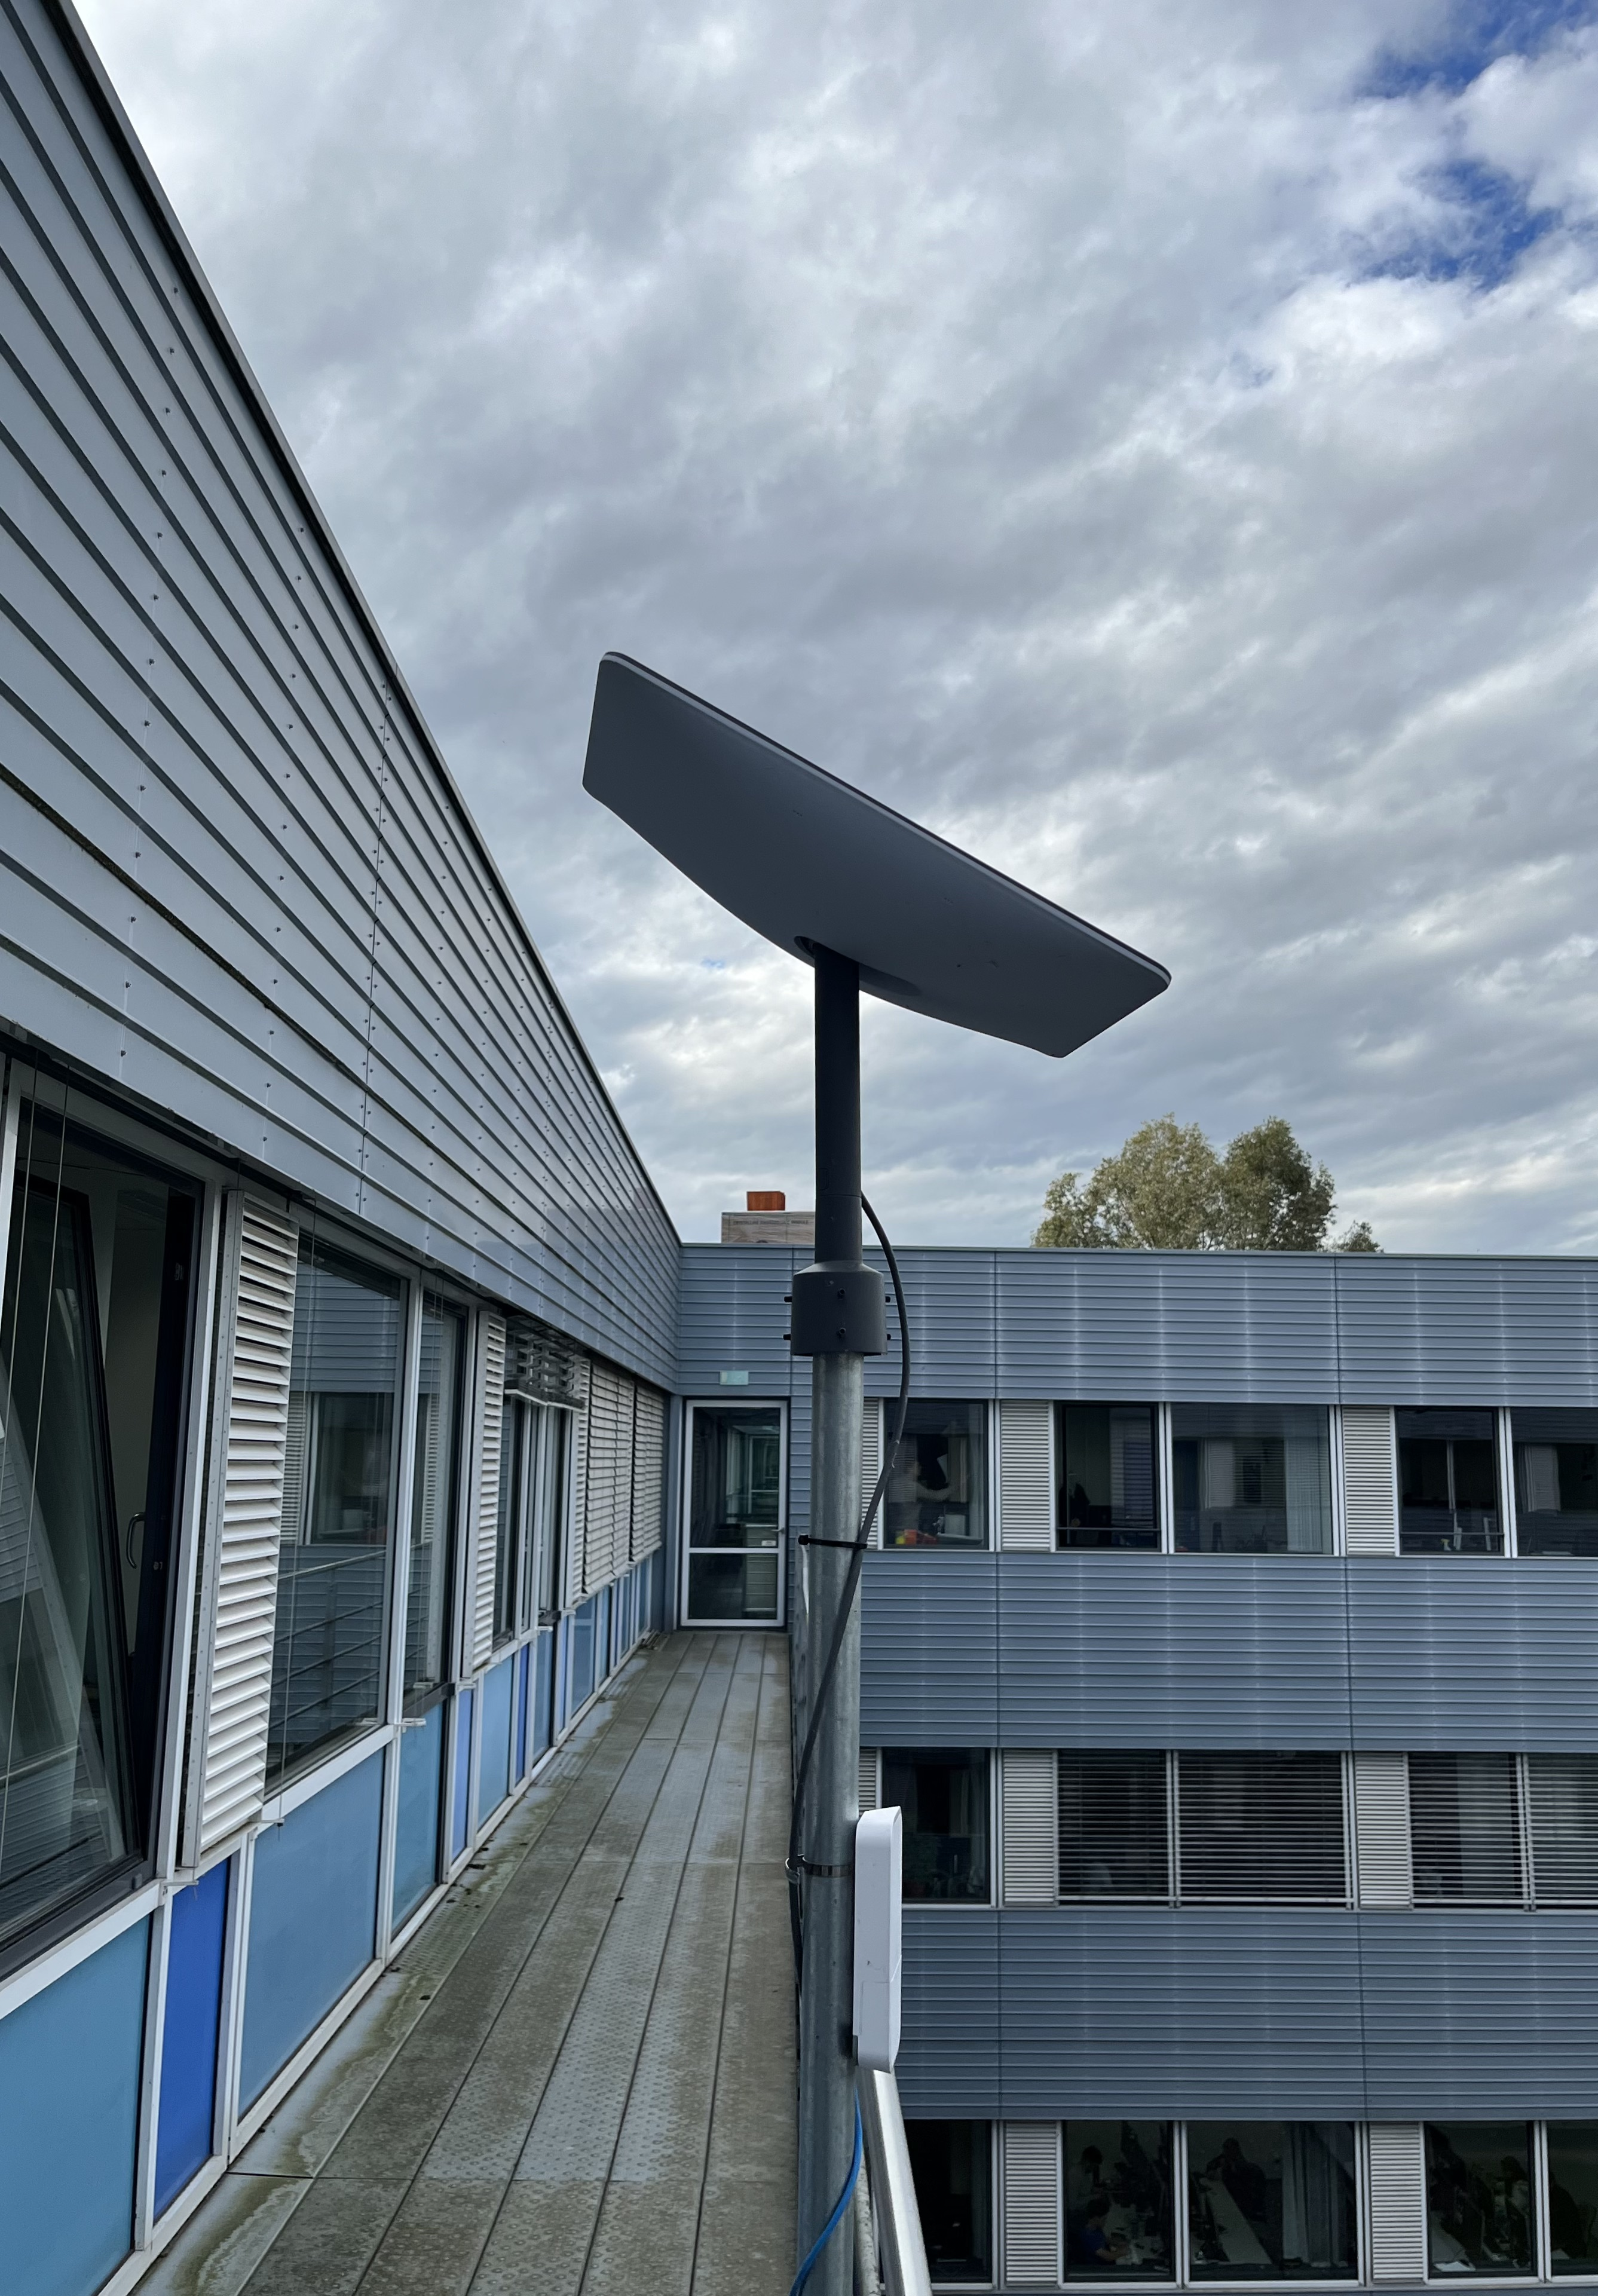
\includegraphics[width=0.6\columnwidth]{img/dish.jpeg}
	\caption{the dish, from Starlink webite Starlink working, from \cite{izhikevich2023democratizing}}
\end{figure}

\begin{figure}
	\label{fig:starlink-101}
	\centering
	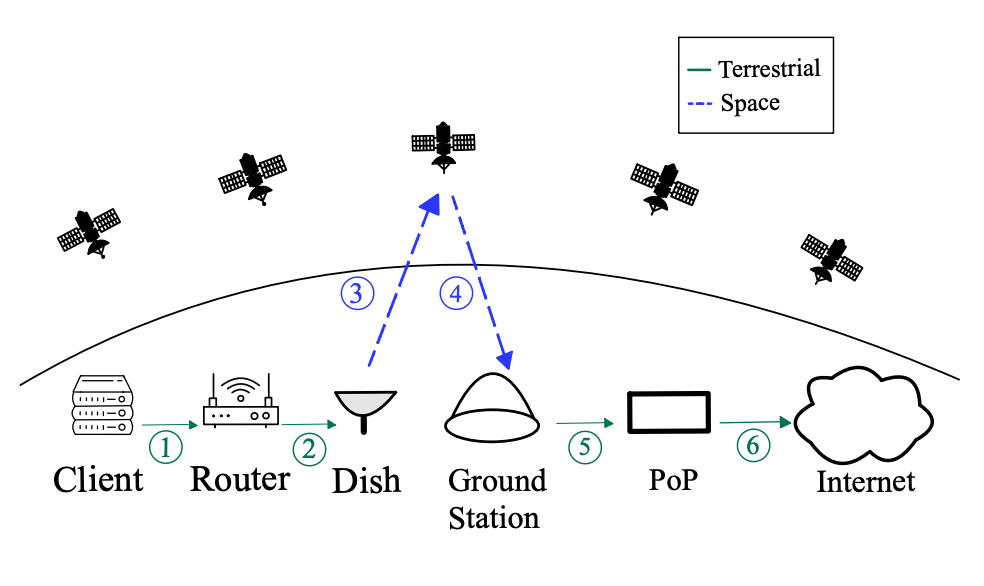
\includegraphics[width=0.6\columnwidth]{img/starlink-101.png}
	\caption{Basic Starlink working, from \cite{izhikevich2023democratizing}}
\end{figure}

SpaceX is currently the most popular LEO-based Internet Service Provider, but other similar projects exist, such as OneWeb \footnote{https://oneweb.net/} and Amazon Project Kuiper \footnote{https://www.aboutamazon.com/what-we-do/devices-services/project-kuiper}, the former one is more enterprise and government focused, while Project Kuiper aims to compete with Starlink.

\chapter{Related work}

durumeric


\chapter{Measurements}

\section{Routing}

\section{Bandwidth analysis}
During our investigations we decided to analyze bandwidth for two reasons: the first one is we wanted to check wheter the data from the API was correct and later to investigate whether we could detect any patterns in bandwidth drops. From \cite{llc-application} we know the dish is seeking for better connections as satellites move constantly each 15 seconds. We plotted the data and tried to verify whether we saw something.
To get the "real" bandwidth we are simply getting data from \texttt{/sys/class/net/{interface}/statistics/rx\_bytes} and dividing it by a factor to get bandwidth in bits per second.

\begin{figure}
	\label{fig:vis-bw-15sec}
	\centering
	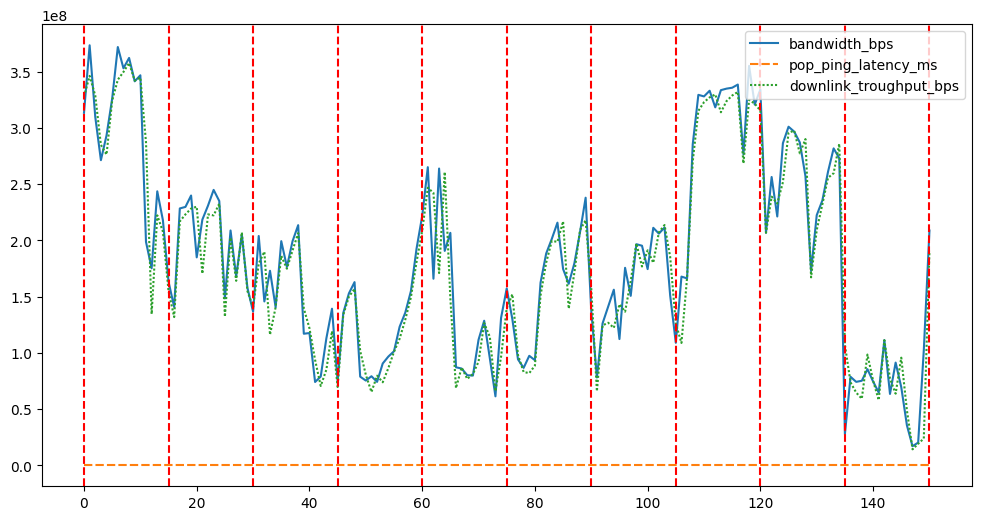
\includegraphics[width=1\columnwidth]{img/bw-15seconds.png}
	\caption{Visualizing bandwidth, \texttt{bandwidth\_bps} is the data we obtain from \texttt{/sys/class/net/{interface}/statistics/rx\_bytes}, while \texttt{downlink\_throughput\_bps} is the data reported from the gRPC api. Additionally we are drawing a vertical red line each 15 seconds.}
\end{figure}

We repeated the experiments shifting the red vertical lines and changing the intervals for collected data, and in the majority of cases we can see that whenever we draw a vertical red line we have some drop in the immediate milliseconds before or after, however drops also happen in different intervals, further investigation might be needed.


\chapter{Satellites}
\label{chap:sats}

In this chapter we will focus on Satellites
\section{Two-line Element Sets}
Two-line Element Sets (hereinafter TLEs) are a widely used data format to encode the postion of orbital elements for a given point in time (WIKIPEDIA). This data format is ASCII based and it will allow us to understand patterns in satellite appearances and to plot the number of visible satellites at any given time. This may be a good substitute for the originally working solution, which was to make a query to retrieve the satellite the dish was connected to. Unfortunately in an earlier phase it might have been possible to call the \texttt{dish\_get\_context} or similar methods that currently either return a \texttt{PermissionDenied} error, or are deprecated.

\begin{lstlisting}[caption={TLE for satellite STARLINK-1007 },captionpos=b]
STARLINK-1007           
1 44713U 19074A   23239.65120160  .00022666  00000+0  15354-2 0  9991
2 44713  53.0553  19.2809 0001296  68.3392 291.7735 15.06406564209327
\end{lstlisting}

	
\section{Skyfield Library}

In order to work with TLEs from the Starlink constellation with Python we are using https://rhodesmill.org/skyfield/, an elegant astronomy library for Python. Retrieving TLEs for every single satellite in the LEO constellation is just a matter of running the following script:

\begin{lstlisting}[language=python,caption={retrieving a Satellite's position using the Satname},captionpos=b]
from skyfield.api import load, wgs84

stations_url = "https://celestrak.org/NORAD/elements/gp.php?GROUP=starlink&FORMAT=tle"
satellites = load.tle_file(stations_url)
print("Loaded", len(satellites), "satellites")
by_name = {sat.name: sat for sat in satellites}
satellite = by_name["STARLINK-1007"]

# year, month, day, hour, minute, second
ts = load.timescale()
t = ts.now()
a = satellite.at(t)
lat, lon = wgs84.latlon_of(a)
print("Latitude:", lat)
print("Longitude:", lon)
\end{lstlisting}

This is a very powerful mechanism, because it allows us to retrieve the satellites we might reasonably assume the dish sees at any given moment.
\subsection{Visible Satellites}
It is up to us to define what "visible" means, in our evaluations we decided that, knowing the satellites orbit around the earth at around 550 kms in height it is reasonable to assume a satellite is visible when it is above the horizon and it is (point to point) not further than 800 kms. The ground truth might be different, but this approximation allows us to approximately have an idea about what is going on in space. 

The first measurement we are setting up is the following: every 15 seconds we run a script that gets all the "visible" satellites and we store them in a SQLite database, if we saw the same satellite in the iteration before we simply update the \texttt{timestamp}, otherwise we create a new row in the db. We use a \texttt{relative\_ts} (relative timestamp) to enumerate every measurement (a probe every 15 seconds). To measure visible satellites we are running the following command: \texttt{python3 visible-satellites.py -v -lat 48.2489 -lon 11.6532 -el 0 -d 800}, where \texttt{lat} and \texttt{lon} are Garching's coordinates, we are not interested in using an elevation.


\section{Patterns in Satellites Appearances}
After having collected data for several hours we decided to plot satellite appearances to check whether they were following some patterns, it seems like it is the case, as you can see in Figure \ref{fig:vis-sat-pat}. We see the same satellite each 12 hours roughly, for some satellites we notice something that might seem like a change in the pattern, but this is not really true, the interval between the appearances is the same as in the other cases, we are not sure we understand why we are seeing this artifact.

\begin{figure}
	\label{fig:vis-sat-pat}
	\centering
	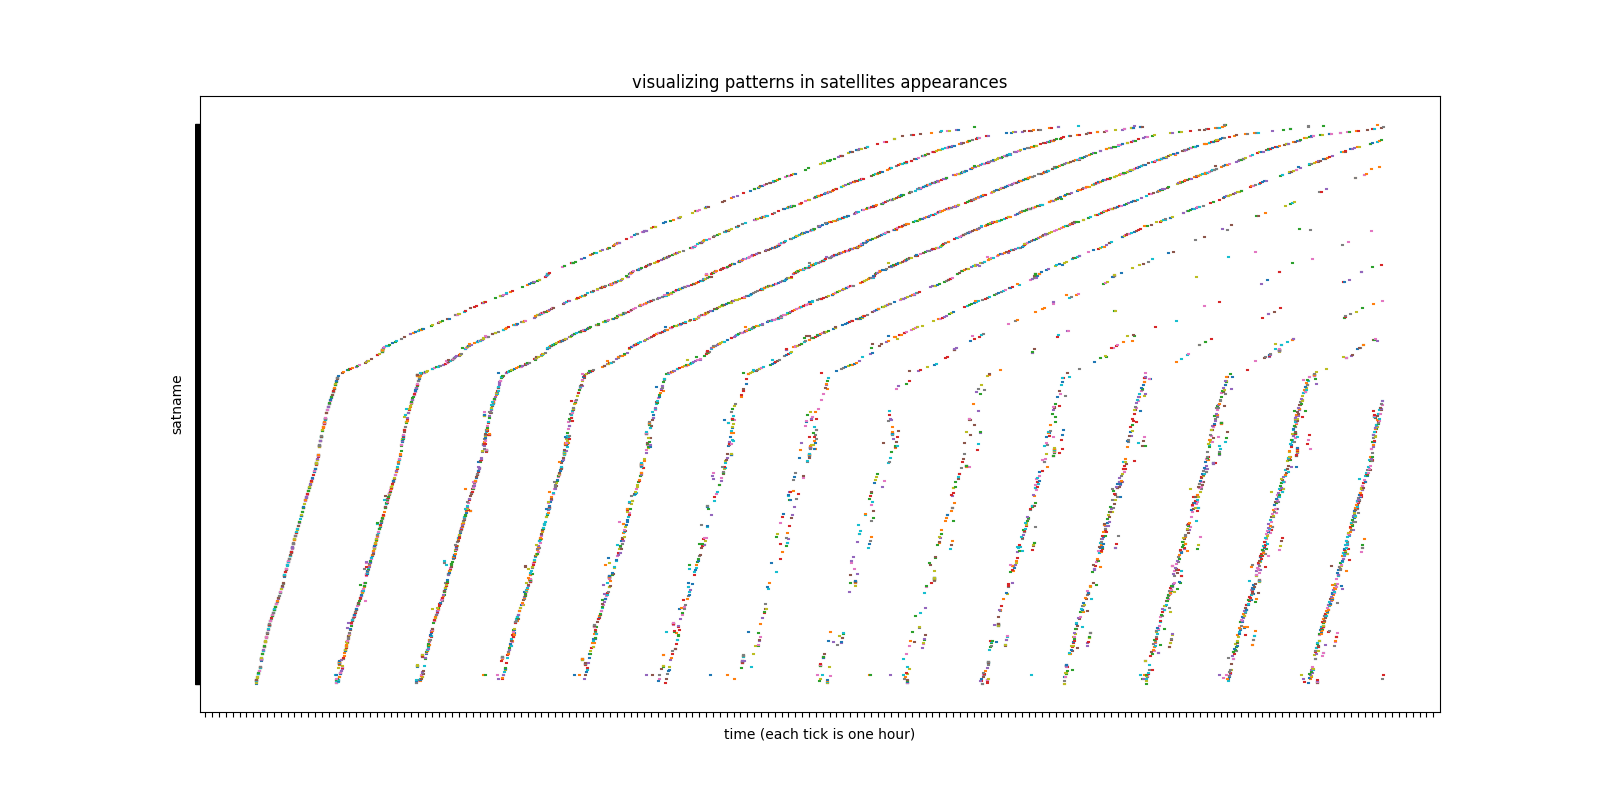
\includegraphics[width=1.2\columnwidth]{img/visualizing-how-long-satellites-are-visible-for.png}
	\caption{Visualizing patterns in satellite appearances, we roughly see the same satellite each 12 hours.}
\end{figure}

\section{Detecting Satellite Handovers}

The Starlink gRPC api exposes a \texttt{dish\_get\_obstruction\_map} method, following the approach described in \cite{izhikevich2023democratizing} we use the information gathered from polling the endpointeach second to extract the current obstruction map and visualize satellite handovers. The reason this works is the dish is adding a dot (setting a value to 1) in a 123*123 matrix whenever it sees a satellite in that position, whenever the dish is rebooted (using i.e \texttt{nine981.reboot}) the matrix is cleared by setting every entry to -1, whenever a satellite is detected the entry is set. By polling the endpoint frequently enough we can observe satellites traces, by comparing values in the matrices we obtain we can detect whether a satellite handover was performed.

\[

\begin{bmatrix}
-1 & -1 & 1 & -1 & -1 \\
-1 & -1 & -1 & 1 & -1 \\
-1 & -1 & -1 & -1 & -1 \\
-1 & -1 & -1 & -1 & -1 \\
-1 & -1 & -1 & -1 & -1 \\
\end{bmatrix}
+
\begin{bmatrix}
-1 & -1 & 1 & -1 & -1 \\
-1 & -1 & -1 & 1 & -1 \\
-1 & -1 & -1 & -1 & 1 \\
-1 & -1 & -1 & -1 & -1 \\
-1 & -1 & -1 & -1 & -1 \\
\end{bmatrix}
=
\begin{bmatrix}
-2 & -2 & 2 & -2 & -2 \\
-2 & -2 & -2 & 2 & -2 \\
-2 & -2 & -2 & -2 & 0 \\
-2 & -2 & -2 & -2 & -2 \\
-2 & -2 & -2 & -2 & -2 \\
\end{bmatrix}
\]

\captionof{figure}{Let's assume these matrices come from the endpoints at $t_x$ and $t_{x+1}$ respectively, in the first matrix we have ones in $(0,2)$ and $(1,3)$, in the second one we have ones in $(0,2)$, $(1,3)$, $(2,4)$, this means the new satellite we saw at $t_{x+1}$ is on the same path as the satellites before, thus NO handover was not performed.}



\[
\begin{bmatrix}
-1 & -1 & 1 & -1 & -1 \\
-1 & -1 & -1 & 1 & -1 \\
-1 & -1 & -1 & -1 & -1 \\
-1 & -1 & -1 & -1 & -1 \\
-1 & -1 & -1 & -1 & -1 \\
\end{bmatrix}
+
\begin{bmatrix}
-1 & -1 & 1 & -1 & -1 \\
-1 & -1 & -1 & 1 & -1 \\
-1 & -1 & -1 & -1 & -1 \\
-1 & -1 & -1 & -1 & -1 \\
1 & -1 & -1 & -1 & -1 \\
\end{bmatrix}
=
\begin{bmatrix}
-2 & -2 & 2 & -2 & -2 \\
-2 & -2 & -2 & 2 & -2 \\
-2 & -2 & -2 & -2 & -2 \\
-2 & -2 & -2 & -2 & -2 \\
0 & -2 & -2 & -2 & -2 \\
\end{bmatrix}
\]
\captionof{figure}{If instead the new satellite we see at $t_{x+1}$ is in a totally different area an handover must have been performed.
}


We can observe it is pretty easy to detect whether an handover was performed, it is sufficient to sum the two matrices and check whether the $0$ value (there was -1 before and we currently have 1) is near an entry whose value is $2$ (at $t_{x}$ value was 1 and at $t_{x+1}$ value is $1$. 



First of all we need to write a script to extract obstruction maps from the dish, to achieve this goal we can use the \texttt{nine981.get\_obstruction\_map} function, this returns a json file similar to this:

\begin{lstlisting}[caption={data from the \texttt{dish\_get\_obstruction\_map} function},captionpos=b]

{'apiVersion': '9',
 'dishGetObstructionMap': {'minElevationDeg': 10.0,
                           'numCols': 123,
                           'numRows': 123,
                           'snr': [-1.0,
                                   -1.0,
                                   -1.0,
                                   1.0,
                                   1.0,
                                   -1.0,
                                   -1.0,
				...,
                                   1.0,
                                   1.0,
                                   1.0,
                                   -1.0,
                                   -1.0,
                                   -1.0,
                                   -1.0]}}  
\end{lstlisting}

Thus we can simply extract the values in \texttt{map["dishGetObstructionMap"]["snr"]} and we can reshape the array in a $123\times123$ with \texttt{np.array(map).reshape(123, 123)}. This allows us to simply visualize the obstruction map at any given moment, it simply a matter of loading the json file we want to visualize and plot it with matplotlib.

\begin{lstlisting}[language=python,caption={visualizing a single obstruction map},captionpos=b]

import json
import numpy as np
import matplotlib.pyplot as plt

f = "1692089163.json"
map = json.load(open(f))
map = map["dishGetObstructionMap"]["snr"]
map = np.array(map).reshape(123, 123)
plt.imshow(map)
plt.show()
\end{lstlisting}


\begin{figure}
	\label{fig:vis-single-map}
	\centering
	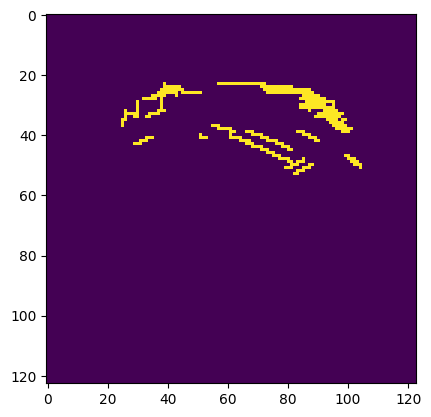
\includegraphics[width=0.5\columnwidth]{img/single_map.png}
	\caption{Visualizing a single obstruction map.}
\end{figure}


Following this approach we can create a simple script to retrieve maps each second and save them locally, later we can export images and create a video to better analyze what is going on. 

We created a simple script to algorithmically detect handovers, we can use the function \texttt{common.detect\_handovers} to detect whether and handover was performed between two subsequent snaphsots, getting all the handovers is simply a matter of iterating for every json file we saved and running the function on each pair.

We now try to correlate satellite handovers (the vertical dashed lines) with the bandwidth measurements we obtained before, our assumption is we might have drops in bandwidth during handovers. Apparently this does not happen, as we can verify from the following figure.


\begin{figure}
	\label{fig:vis-correlation-handovers}
	\centering
	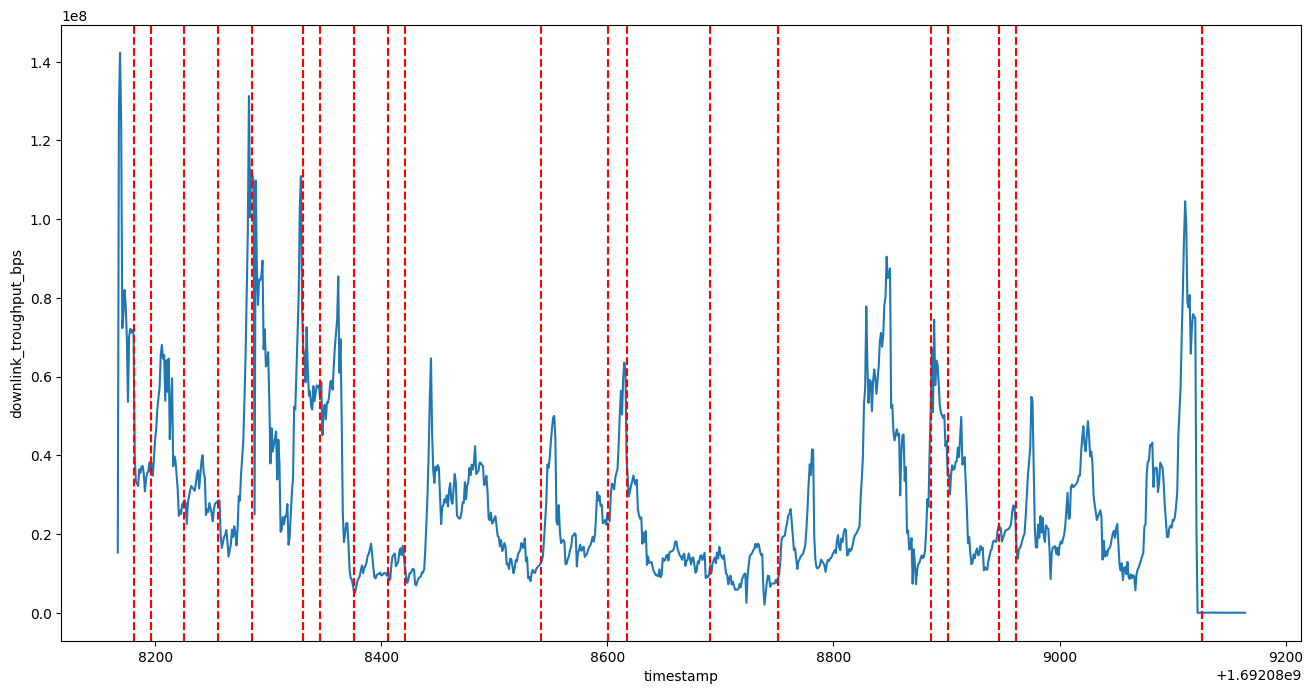
\includegraphics[width=1\columnwidth]{img/correlation_handovers_bw.png}
	\caption{Trying to correlate satellite handovers (red vertical lines) with bandwidth measurements.}
\end{figure}

we should also mention the 15 second intervals
here i will insert a simple demo of the handover detection overlapped to the bandwidth measurements, 



\chapter{Routing}
\section{Cloud Traceroutes}
\section{Tooling}
\section{Visualizing Traceroutes}


\chapter{Exploring the gRPC api}

grcpurl
query all methods
in appendix probably? insert working methods and stuff


\section{Tooling}
\section{Getting Obstruction Maps}
Following the approach sketched in \cite{izhikevich2023democratizing} we started retrieving obstruction maps from the dish using the \texttt{dish\_get\_obstruction\_map} method exposed by the gRPC api on the dish.



\begin{figure}
	\centering
	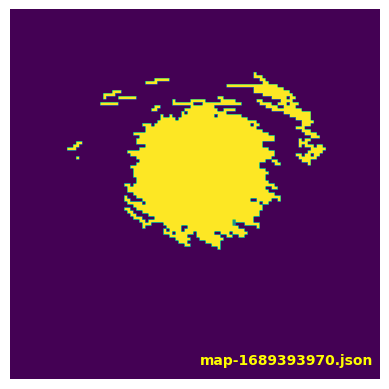
\includegraphics[]{img/obstruction_map_finale.png}
	\caption{An obstruction map retrieved by the dish, check <CITE APPENDIX> to understand how it was generated}
\end{figure}

\chapter{/dev/random}

\section{Introducing some latency measurements}
\section{Does the dish buffer packets?}

After measuring latency and bandwidth we noticed some patterns in bandwidth drops, as per Figure <CITE> 

\begin{figure}
	\centering
	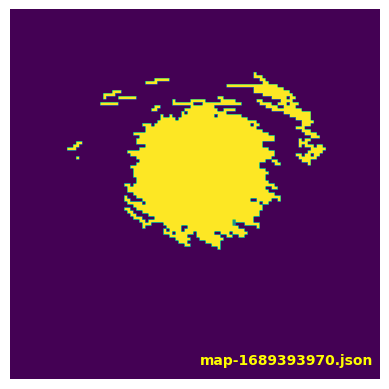
\includegraphics[]{img/obstruction_map_finale.png}
	\caption{An obstruction map retrieved by the dish, check <CITE APPENDIX> to understand how it was generated}
\end{figure}

now we want to assess whether the dish buffers packets relayed to satellites, our intuition is that if this is the case we will see a decrease in RTT if we start creating some traffic with a tool like iperf3 on the very same interface

mesurements with  curl --interface enp1s0f3 http://ftp.uio.no/debian-cd/12.1.0-live/amd64/iso-hybrid/debian-live-12.1.0-amd64-lxde.iso > /dev/null

\appendix
\chapter{Appendix}
\label{chap:appendix}

\section{Appendix section}

\begin{lstlisting}[language=python,caption={the \texttt{calculate\_visible\_satellites} function},captionpos=b]
def calculate_visible_satellites(
    observer_latitude, observer_longitude, observer_elevation, distance_km
):
    stations_url = (
        "https://celestrak.org/NORAD/elements/gp.php?GROUP=starlink&FORMAT=tle"
    )

    satellites = load.tle_file(stations_url)
    observer = Topos(observer_latitude, observer_longitude, observer_elevation)
    ts = load.timescale()
    t = ts.now()

    # Calculate satellite positions
    positions = []
    for sat in satellites:
        satellite = sat
        position = (satellite - observer).at(t)
        positions.append((sat, position))

    # Filter visible satellites
    visible_satellites = []
    for sat, position in positions:
        alt, az, distance = position.altaz()
        # Satellite is above the horizon
        if alt.degrees > 0 and distance.km < distance_km:
            visible_satellites.append((sat, alt, az))

    return visible_satellites
\end{lstlisting}

The appendix can contain different sections.

\clearpage
\pagestyle{thesischapter}

\cleardoublepage
\selectlanguage{english}

\printbibliography[heading=bibintoc]
%\cleardoublepage
\clearpage
\pagestyle{empty}
%\mbox{}
%\clearpage

\end{document}
 